\subsection{Measuring Master von Bosch}

\subsubsection{Vorstellung}
\todo{Version, Downloaddatum, Playstore-Link}
Die App \emph{Measuring Master} von der Bosch GmbH ist im Play-Store unter der Rubrik ``Effizienz'' aufgelistet.
Selbst beschreibt der App-Hersteller seine Software wie folgt \citep{BoschMM}:

\begin{quote}
  ``Measuring Master ist eine multifunktionale App, die es ermöglicht, Aufmaße, Grundrisse und Temperaturmesswerte an einem Ort zu dokumentieren und zu verwalten.\\
  Die App ist besonders geeignet für Architekten, Maler, Bodenleger, Heizungsbauer und Elektriker, aber auch alle anderen Handwerker profitieren von der umfangreichen Funktionalität''
\end{quote}

\noindent
Nach dem Start der Applikation bietet sich die Möglichkeit ein neues Projekt anzulegen, oder bereits vorhandene Projekte zu bearbeiten.
Sobald das gewünschte Projekt ausgewählt wurde, bieten sich dem Benutzer über das Menü an der linken Seite diverse Funktionen (siehe \autoref{fig:bmenu}) an. \\

\begin{figure}[h]
  \centering
	\begin{subfigure}[b]{0.4\textwidth}
		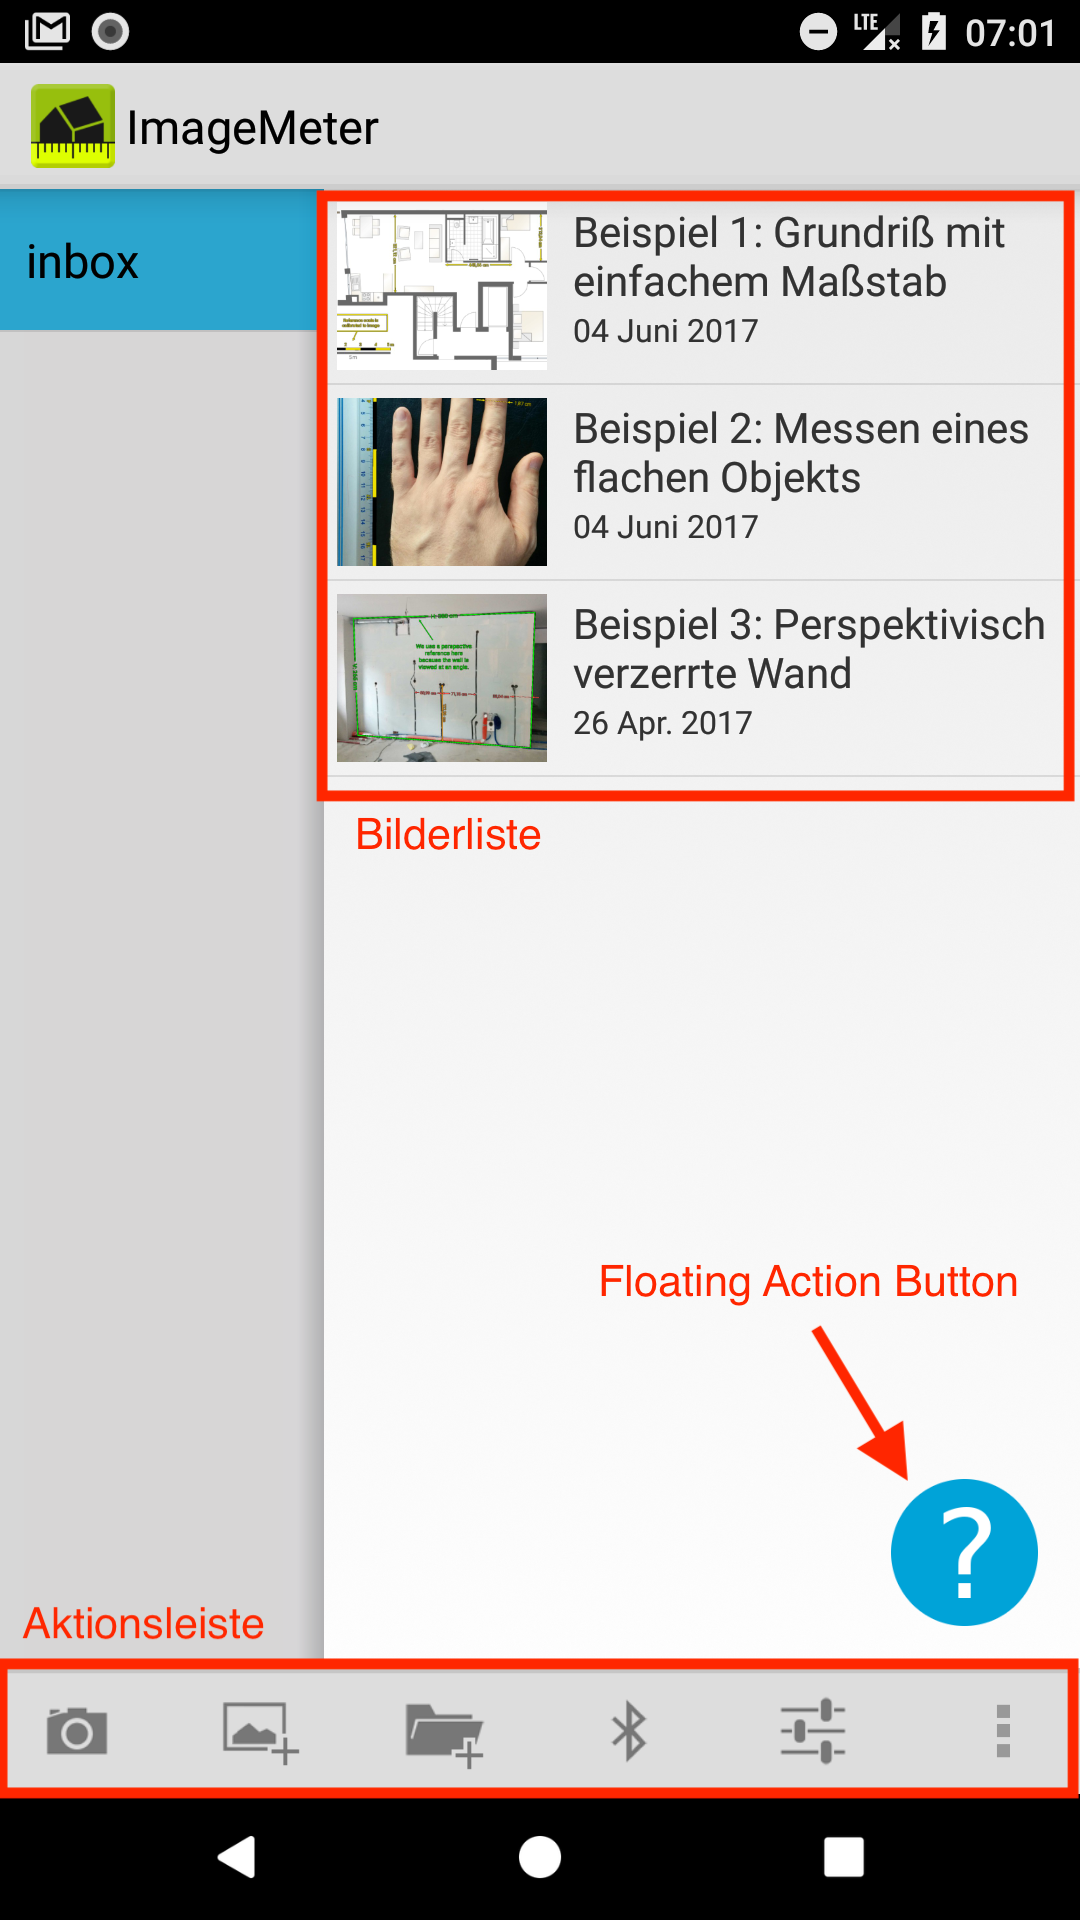
\includegraphics[keepaspectratio, width=\textwidth]{bosch/menu}
		\caption{Navigationsmenü}
		\label{fig:bmenu}	
	\end{subfigure}
	\begin{subfigure}[b]{0.4\textwidth}
		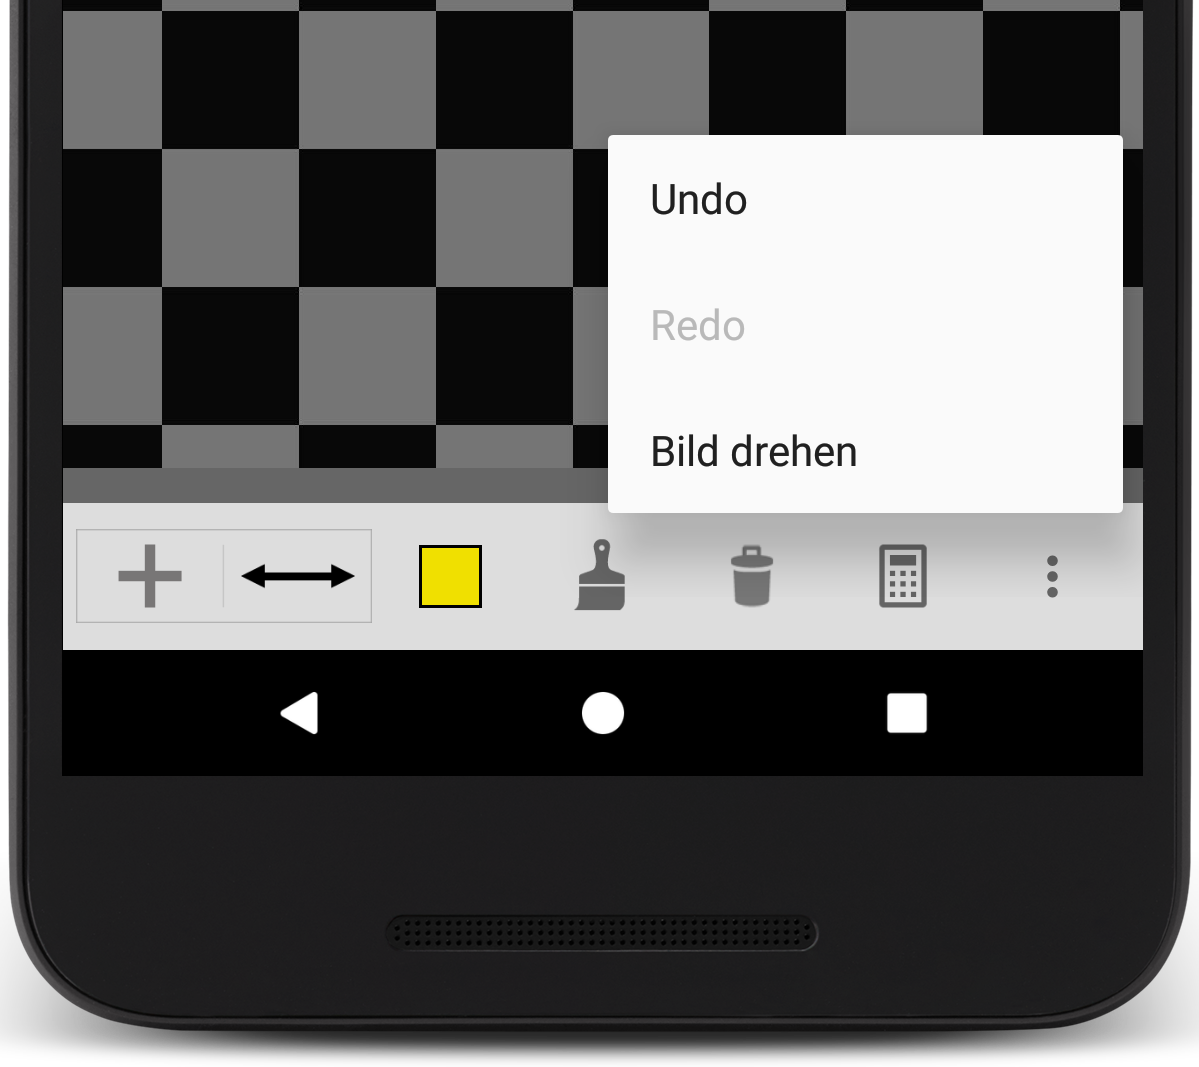
\includegraphics[keepaspectratio, width=\textwidth]{bosch/bar}
		\caption{Aufmaße-Funktion}
		\label{fig:bbar}	
	\end{subfigure}
  \caption{Measuring Master bei ausgeklapptem Navigationsmenü und in der Aufmaße-Funktion}
\end{figure}

Im Folgenden wird der Menüpunkt ``Aufmaße'' und die damit verbundene Funktionalität weiter vorgestellt und evaluiert.
So bietet sich dem Benutzer nach Auswahl der Aufmaße-Funktion die Möglichkeit, ausgewählte Bilder direkt mit Messwerten zu beschriften.
Hierzu können entweder Bilder direkt aus der Gallerie importiert, oder mit der Kamera aufgenommen werden.
Sobald der Benutzer den Foto-Import erfolgreich abgeschlossen hat, öffnet sich eine neue Ansicht, welche das ausgewählte Bild und weitere Bedienelement, in Form einer Statusleiste am unteren Rand, zeigt (siehe \autoref{fig:bbar}). \\

In dieser Benutzeroberfläche kann der Nutzer mit Hilfe von vier verschiedenen Formen (Linie, Viereck, Winkel, Freiform) Aufmaße ins Bild anzeichnen, und über einen Klick auf die gewünschte Form, Messwerte eintragen.
Außerdem bietet die App die Option, eine ausgewählte Reihe von Laserentfernungsmesser mit der App zu verbinden.
Dies ermöglicht eine Übertraung der gemessenen Distanzen über eine Bluetooth-Schnittstelle direkt an die App. \\

Um das annotierte Bild außerhalb der App weiter zu benutzen, bietet diese den Export als \emph{PDF} und \emph{JPEG} an.
Die exportierte \emph{PDF} enthält im Gegensatz zu der \emph{JPEG} zusätzlich zu dem annotierten Bild auch noch eine Tabelle mit allen eingetragenen Messwerten \autoref{fig:bexport}. 
Zudem lassen sich annotierte Bilder in der App speichern und zu einem späteren Zeitpunkt wieder bearbeiten.

\begin{figure}[h]
  \centering
  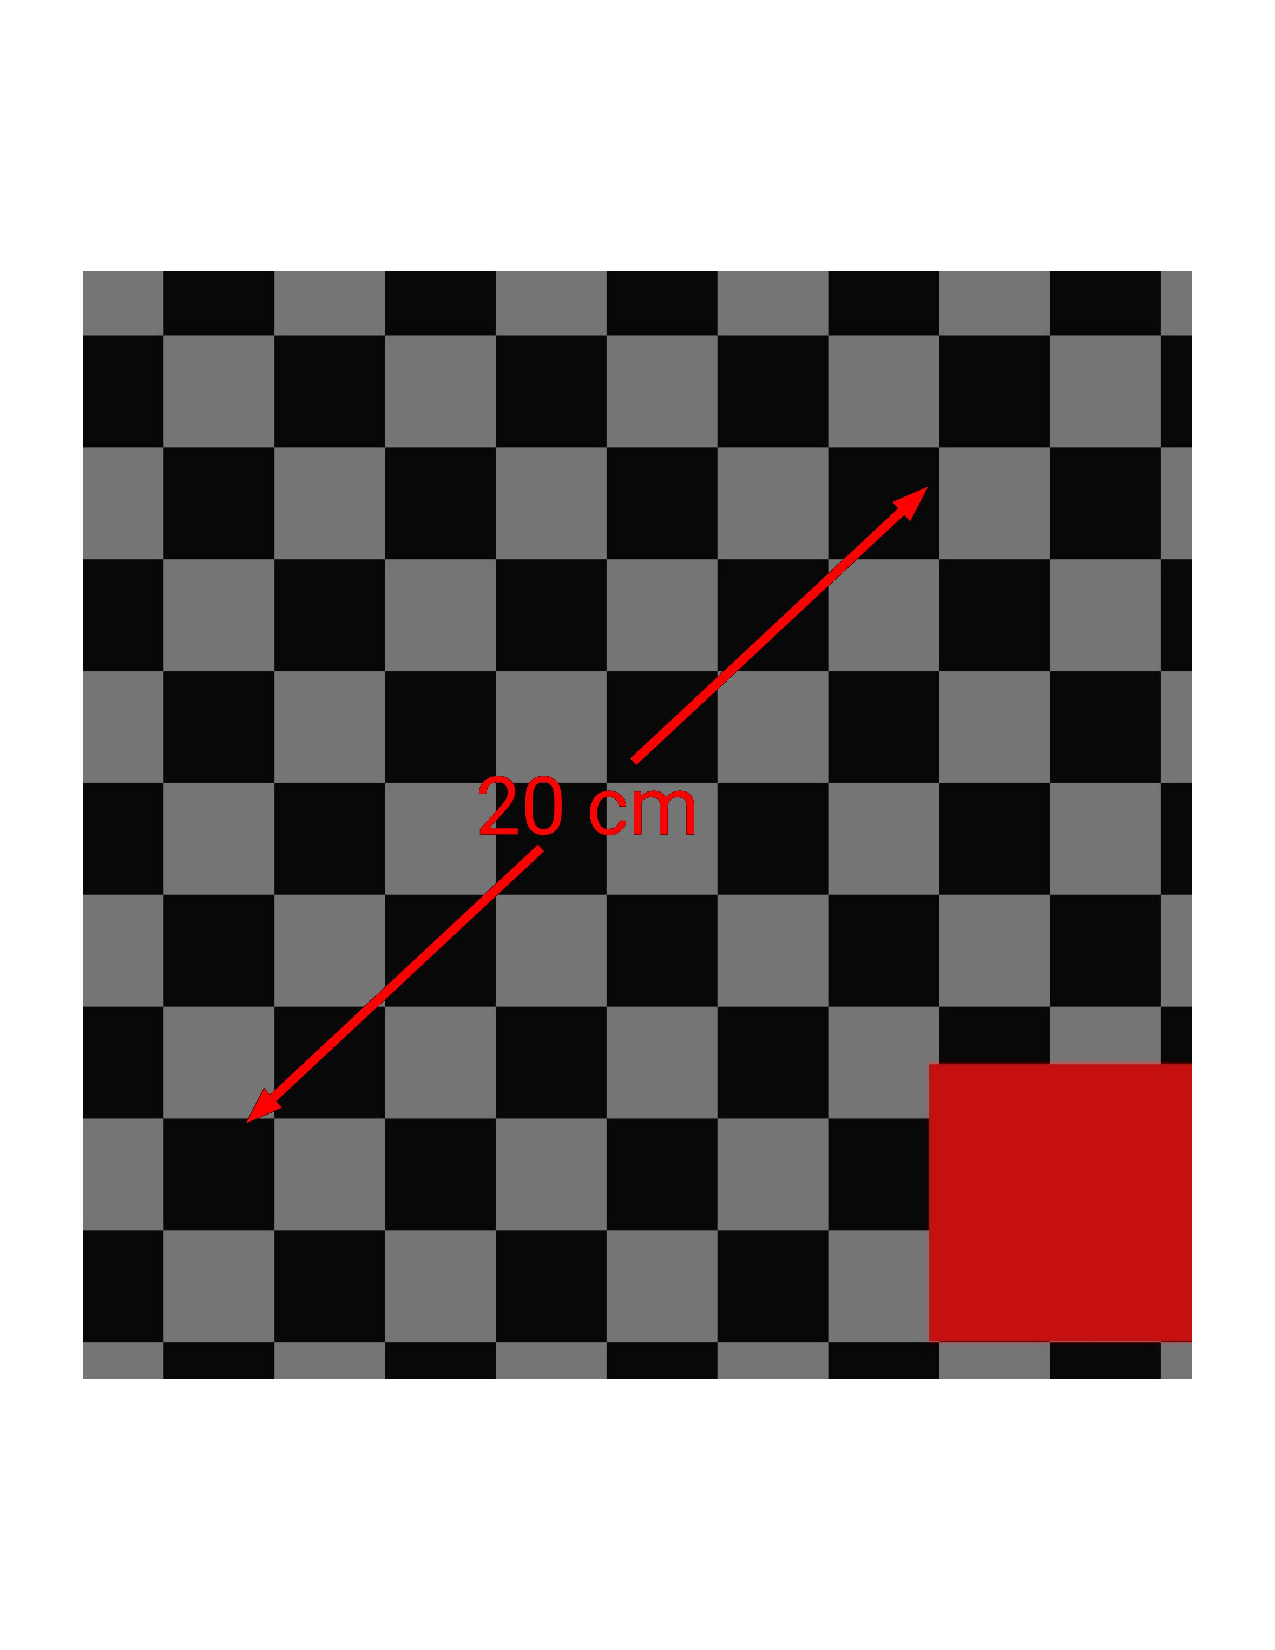
\includegraphics[keepaspectratio, width=\textwidth]{bosch/export}
  \caption{Exportierte PDF}
  \label{fig:bexport}
\end{figure}

\subsubsection{Evaluation}

Die App zeigt in einer Art Statusleiste am unteren Rand des Bildschirms den aktuellen Modus an, und gibt über einen auffordernden Text am oberen Bildschirmrand dem Nutzer eine Hilfestellung, was er im gerade ausgewählten Modus machen kann. \todo{screens} Hiermit deckt die App Nielsen \ref{itm:1} und \ref{itm:10} ausreichend ab. \\

Des Weiteren benutzt auch diese App universell verständliche Icons, um die wichtigsten Aktionen wiedererkennbar zu machen. So hat beispielsweise das Mülleimer-Icon in jedem Modus die Löschfunktion. \\

Im Gegensatz zu \textsc{Photo Measures} bietet diese App dem Benutzer die Möglichkeit seine Aktionen rückgängig zu machen, oder sie zu wiederholen. Dies ist ein deutlicher Vorteil seitens der Usability, da Fehler nicht so hart bestraft werden, als wenn keine Undo/Redo-Button vorhanden wären. \\

Fehler werden hier durch das Deaktivieren von Buttons, die im aktuellen Systemzustand nicht benutzbar sind, präventiv verhindert. Das Löschen von Formen ist beispielsweise nur dann möglich, wenn zuvor eine Form ausgewählt wurde.

Negativ fällt auch in dieser Alternative die fehlerhafte Gesten-Unterstützung auf. So sorgen Zoom-Gesten per Doppel-Tap zum unabsichtlichen Zeichnen einer Form, welche im Nachhinein wieder gelöscht werden muss. Außerdem verletzt die App Nielsen~\ref{itm:15}, da Änderungen in der Bildschirmausrichtung dafür sorgen, dass das Bild nicht wie erwartet seine Ursprungsausrichtung beibehält, sonder auch rotiert wird. 

\begin{figure}[h]
	\begin{subfigure}[b]{0.5\textwidth}
		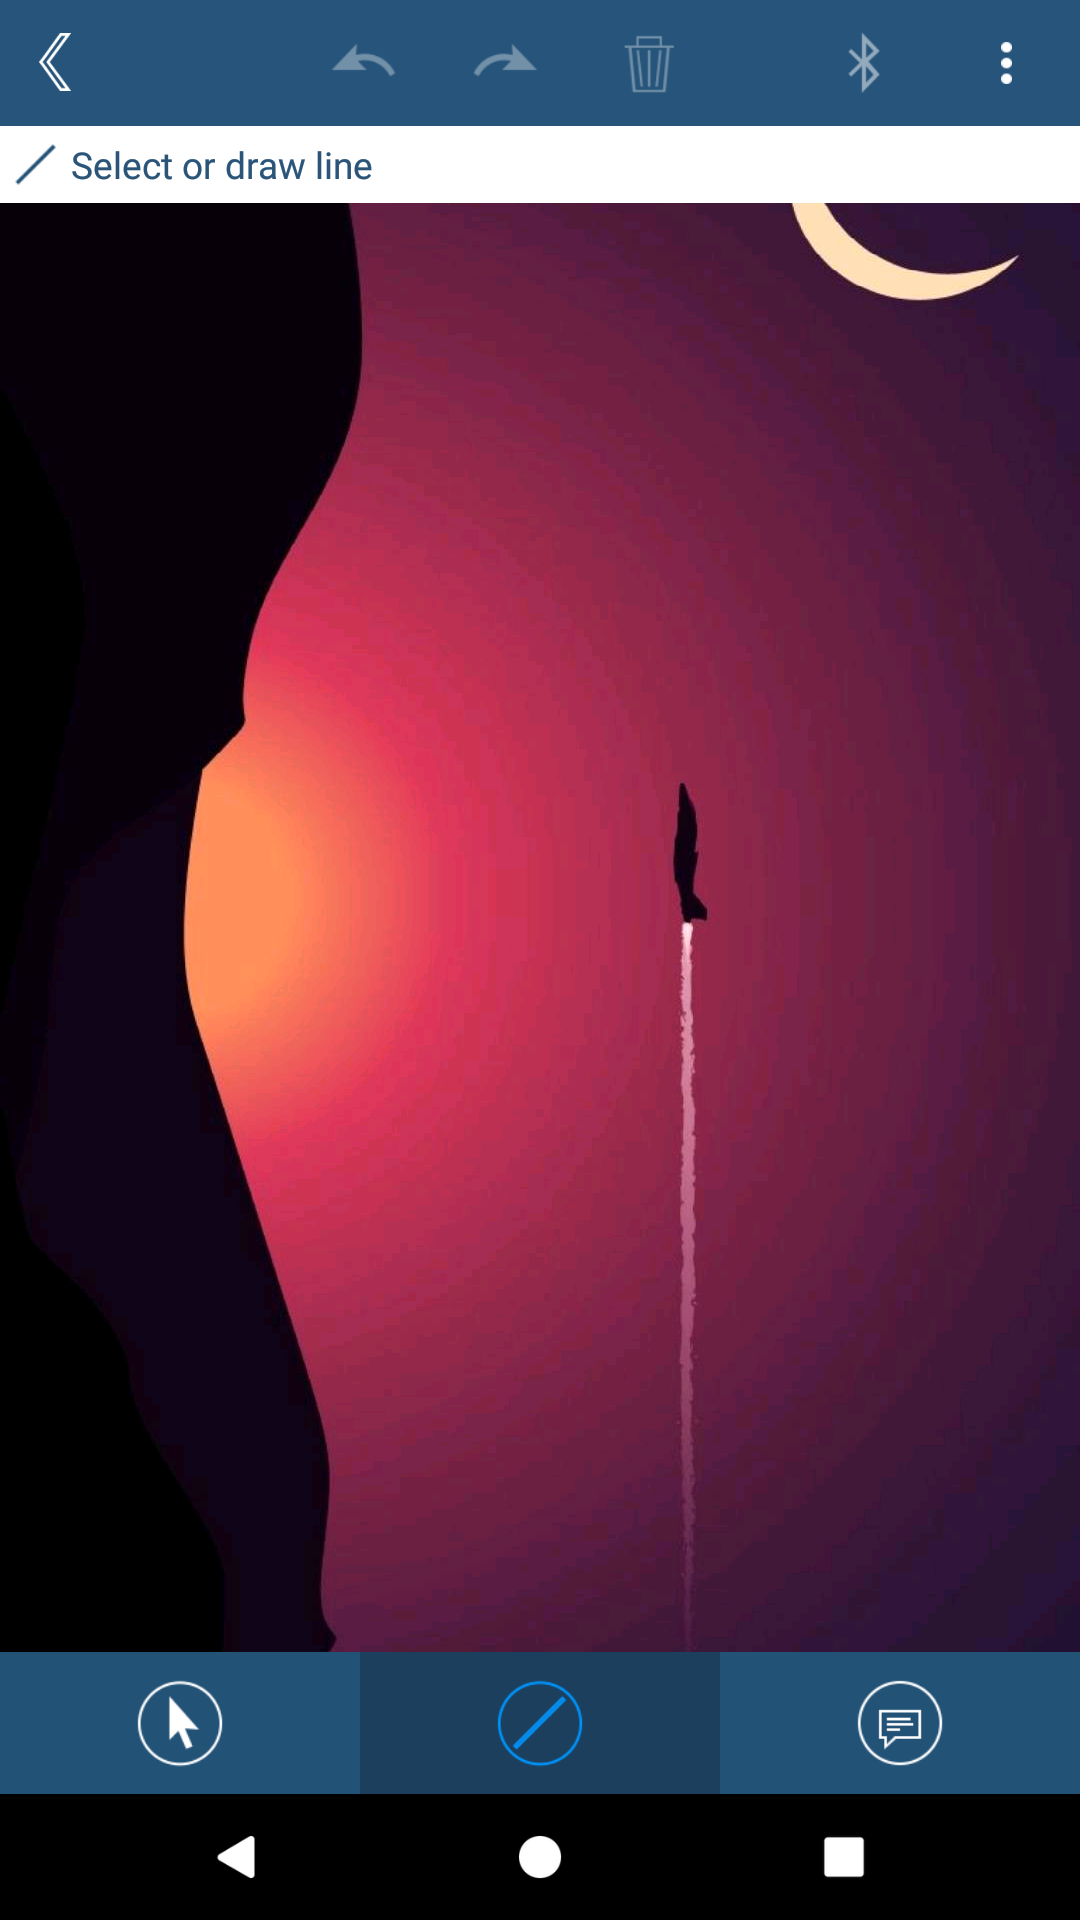
\includegraphics[keepaspectratio, width=0.9\linewidth]{bosch/portrait}
		\caption{App im Portrait-Modus}
		\label{fig:bportait}	
	\end{subfigure}
	~
	\begin{subfigure}[b]{0.5\textwidth}
		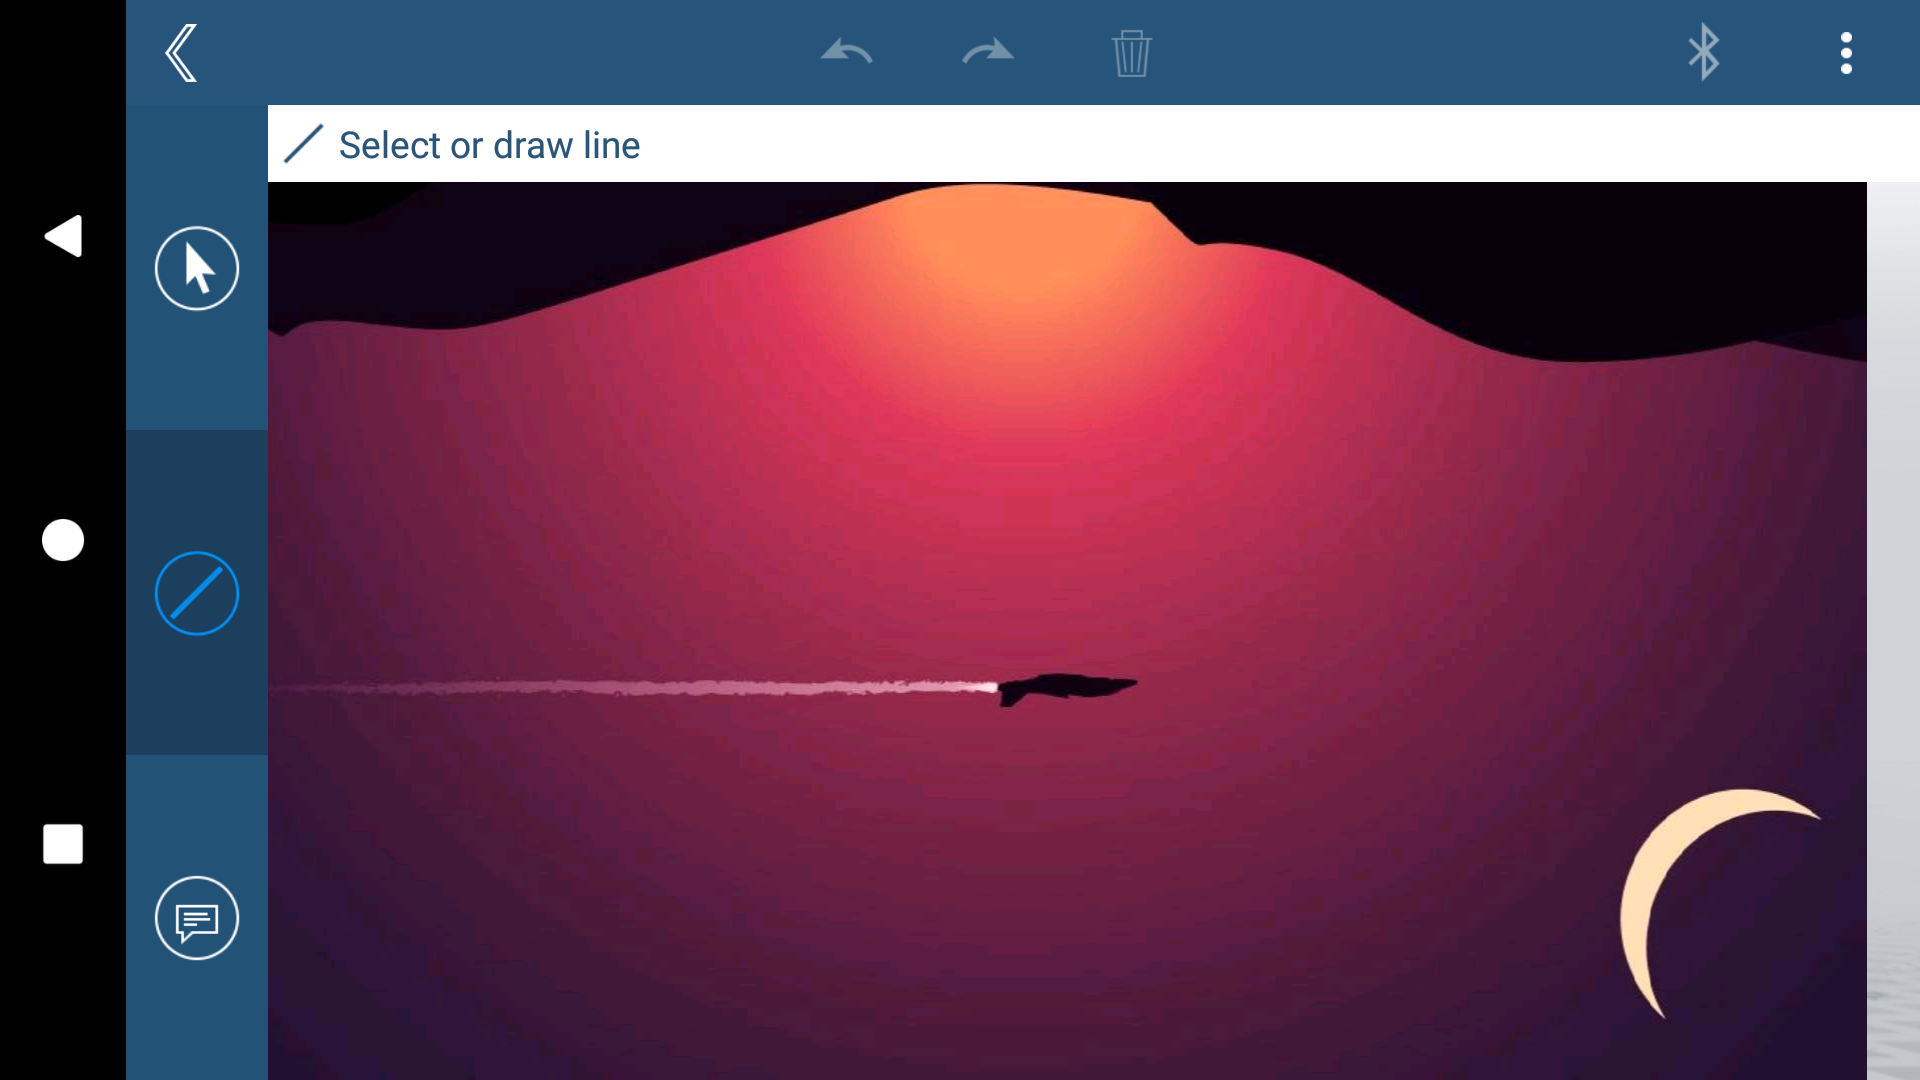
\includegraphics[keepaspectratio, height=0.7\linewidth]{bosch/landscape}
		\caption{App im Landscape-Modus}
		\label{fig:blandscape}	
	\end{subfigure}
	\caption{Bildschirmrotation Bosch-App}
	\label{fig:borientation}
\end{figure}
